\section{Introduction}\label{sec:introduction}
Bayesian inference provides a principled framework for estimating unknown quantities from noisy observations. Conditional normalizing flows provide a way towards amortized Bayesian inference, which means making Bayesian parameter identification reusable across datasets \citep{radev2021amortized}. Trained on simulated parameter--observation pairs, BayesFlow \citep{radev2020bayesflow} combines a learned summary of the observations with an invertible transformation to approximate the parameter posterior. Once fitted, the model produces posterior samples for new observations without repeating parameter optimization. This amortization makes expressive Bayesian inference practical for repeated identification tasks. Its success motivates the question studied here: how can conditional normalizing flows be combined with temporal dynamics to infer evolving states and their uncertainty?

State estimation extends the inference target from a fixed parameter vector to a sequence of unknown states. Noisy or partial measurements constrain that sequence, while temporal dependence links uncertainty at one time to states at subsequent times. A useful estimator must therefore combine flexible conditional distributions, information from the observations, and a model of temporal evolution. Neural stochastic differential equations (SDEs) provide a natural starting point: a learned drift describes nominal evolution, and a stochastic term represents variability around it. 

Latent SDEs \citep{li2020scalable} and SDE-GANs \citep{kidger2021gan} offer two approaches to learning neural SDEs from data. Latent SDEs represent time series through an underlying stochastic process and learn its dynamics through variational inference, coupling a generative SDE with an approximate posterior process. When the observation model uses a Gaussian decoder with learned variance, it can inherit a decoder variance-collapse problem: the estimated variance may approach zero, making training highly sensitive to small reconstruction errors and destabilizing optimization \citep{takahashi2018student,rybkin2021calibrated}. This limitation motivates exploring alternative deep generative models for neural SDEs.

SDE-GANs treat a neural SDE as a trajectory generator and train it against a discriminator to match observed path distributions. This framework accommodates flexible stochastic dynamics, but requires coupled adversarial optimization and careful discriminator regularization \citep{kidger2021gan}. Moreover, it does not directly provide a tractable finite-interval transition likelihood, making it less suited to the likelihood-based conditional state estimation considered here. 

Diffusion models \citep{ho2020denoising} and flow matching \citep{lipman2023flow} provide further approaches to learning expressive generative distributions. One way to apply these methods is to treat an entire state trajectory as a single structured sample and generate its states jointly, as demonstrated by diffusion-based trajectory planning \citep{janner2022planning}. In such formulations, the denoising or transport process evolves in an auxiliary generative time and does not directly parameterize sequential stochastic state updates in physical time. 

Therefore, we seek to combine the temporal structure of neural SDEs with the explicit conditional densities and direct sampling offered by Normalizing Flows \citep{dinh2014nice,rezende2015flows,dinh2017realnvp}. The flow transforms the noise within each state update while preserving tractable likelihoods and the sequential structure of neural SDEs. We call this construction \method. An observation-conditioned neural drift supplies a nominal state update, and an invertible conditional flow transforms Gaussian inputs into state-dependent noise. This design gives nominal evolution and the stochastic increment distribution separate parameterizations, trained jointly from paired state--measurement data. Figure~\ref{fig:overview} shows the resulting estimator.

\begin{figure}[htbp]
\centering
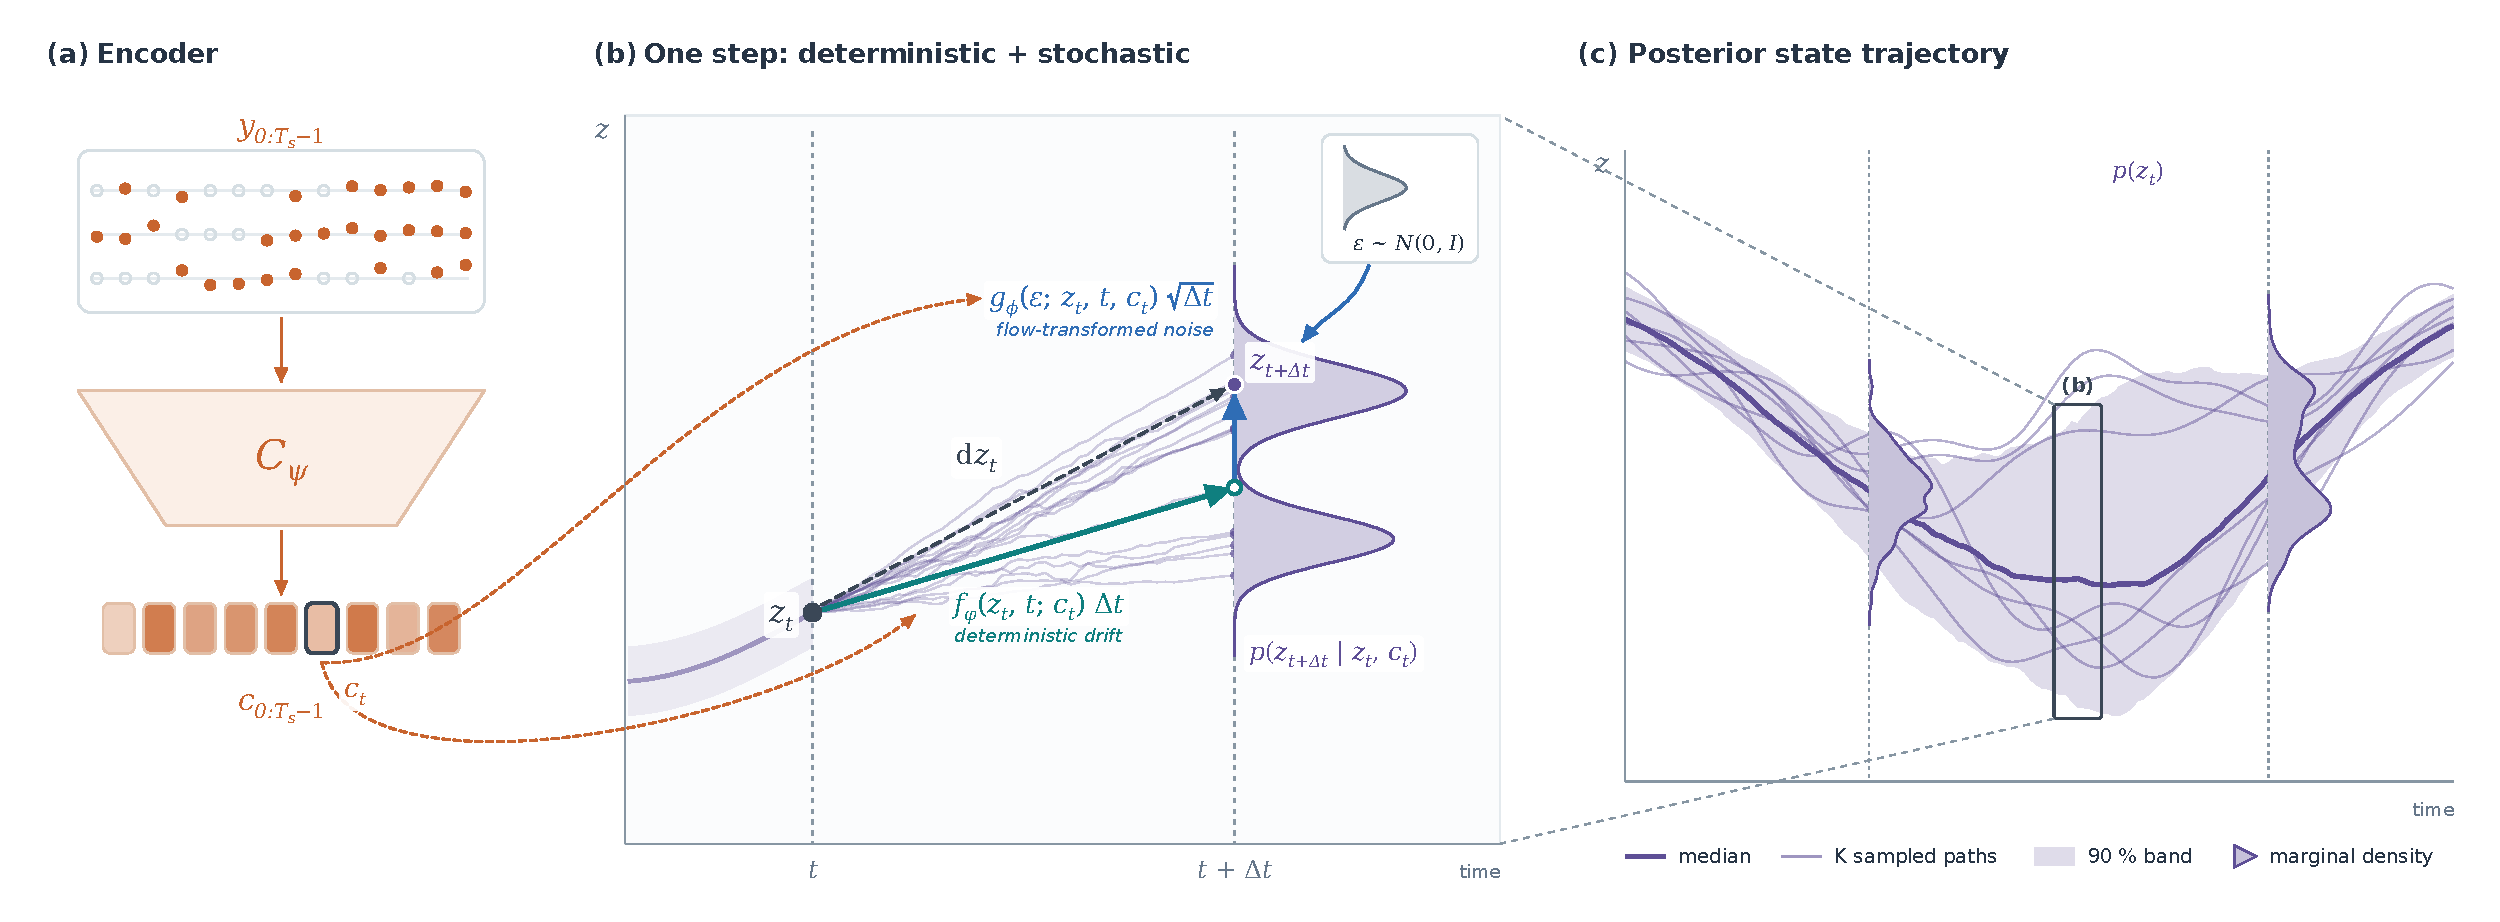
\includegraphics[width=\linewidth]{figures/NormFlowSDE_figure.pdf}
\caption{\method estimates states conditional on observations. (a) At each step, the encoder $C_\psi$ maps a trailing observation window ending before the state being estimated to a context vector $c_t$ (orange), which conditions both the drift and the noise model. The displayed measurement and context arrays summarize these windowwise encodings. (b) Each state update combines a deterministic drift increment (green) with flow-transformed Gaussian noise (blue), yielding a flexible conditional distribution for the next state $z_{t+\Delta t}$ (purple). (c) Repeated updates from the supplied initial state generate $K$ sampled state trajectories; the plot shows their pointwise median, 90\% uncertainty bands, and marginal state densities at selected times. The marginal label $p(z_t)$ leaves the fixed observation windows and controls implicit. The boxed interval is expanded in (b). All curves and densities are schematic.}
\label{fig:overview}
\end{figure}

The construction also raises a mathematical question: under what conditions does the flow-based state update admit a continuous-time SDE limit? In Appendix~\ref{app:diffusion}, we prove that, with the learned coefficients fixed and under explicit regularity and moment assumptions, the trajectories of a centered inference scheme converge in distribution to the unique solution of an It\^o SDE as the time step tends to zero. 

Section~\ref{sec:experiments} evaluates \method as a causal amortized filter on two simulated systems (a controlled pendulum and the Lorenz--96 model) and two robot datasets (ALOHA insertion \citep{zhao2023aloha} and REASSEMBLE \citep{sliwowski2025reassemble}), against three particle filters whose transition and measurement models are learned from the same data: NF-DPF \citep{chen2025flowparticle}, NSF \citep{kiyohara2025nsf}, and FlowSDE \citep{lou2026flowsde}. 
